\chapter{TileCal PMT response}
\label{app:pmt}

\section{Luminosity measurement with TileCal}

The general strategy to measure the luminosity in \gls{atlas} is outlined in Section \ref{sec:lumimeas}.
LUCID is the \gls{atlas} detector that, during \gls{vdm} runs, measures the absolute luminosity. 
LUCID algorithms are non-linear with $\mu$, and this non-linearity is corrected with the calibration transfer, 
that 
allows to extrapolate the absolute LUCID calibration from conditions corresponding to few low-$\mu$, isolated bunches 
to the conditions of the physics runs, where we have many high-$\mu$ bunches in trains. 

The default system used to provide the calibration transfer is track. As already discussed in Section \ref{sec:lumimeas},
the number of reconstructed tracks in the \gls{id} is proportional to $\mu$. 
The track selection that is used for the calibration transfer corresponds to the TightPrimary quality criteria but dropping 
the requirement on the Pixel holes (that have to be $\leq 1$ for the standard TightPrimary selection);
furthermore there is a requirement on the impact parameter significance, $|d_0|/\sigma(d_0)<7$, and on 
the pseudorapidity of the track, $|\eta|<1$. These criteria have been optimized to reduce the dependence on the Pixel conditions. 

The procedure to determine the calibration transfer consists of three steps:
\begin{enumerate}
\item The bunch-averaged track luminosity during the \gls{vdm} run is normalized to the LUCID luminosity (which in these runs 
undergo the absolute calibration). The \gls{vdm} runs have low-$\mu$ isolated bunches.
\item The ratio of the luminosity measured by LUCID and track is measured as a function of $\mu$ (as measured by LUCID) 
in a single run with high-$\mu$ trains. The distribution of the values of this ratio is fitted with a straight line.
\item The result of the fit is used to apply a correction to the luminosity measured by LUCID in physics runs. 
%Fit the relative mu-dependence between the two in a single calibration-transfer run with high-mu trains. In the plot: x-axis mu measured by lucid. y: ratio of track to lucid luminosity. Fit the line. The mu dependence corresponds to an 11\% correction at mu=50 to the lucid response. This is a large number that we have to control at sub-percent level. 
%Apply to LUCID in physics runs 
\end{enumerate}

To assign an uncertainty to the calibration transfer, 



\section{PMT response in empty bunches}
\label{sec:app:pmtresponse}

\section{Impact on calibration transfer uncertainty}

The change in the \gls{pmt} response with the increase in luminosity has a direct implication in the 
\gls{tilecal} luminosity measurement. 
In particular, it means that the increase in measured current with the increase in luminosity comes from 
two distinct factors:
\begin{itemize}
\item The actual increase in luminosity, i.e. having more particles traversing the detector.
\item The increase in \gls{pmt} response.
\end{itemize}

While the first bullet is the effect that we want to measure to provide a luminosity calibration, 
the second bullet has the effect of artificially increasing the \gls{tilecal} 
luminosity measurement. The value of the \gls{pmt} non-linearity measured in Section \ref{sec:app:pmtresponse} 
is used to correct for this undesired effect, with the net result of \gls{tilecal} providing a higher value 
for the luminosity measurement for the \gls{vdm} run, as schematically illustrated in Figure \ref{fig:apppmt:sketch}.


\begin{figure}[ht]
\centering
\subfigure{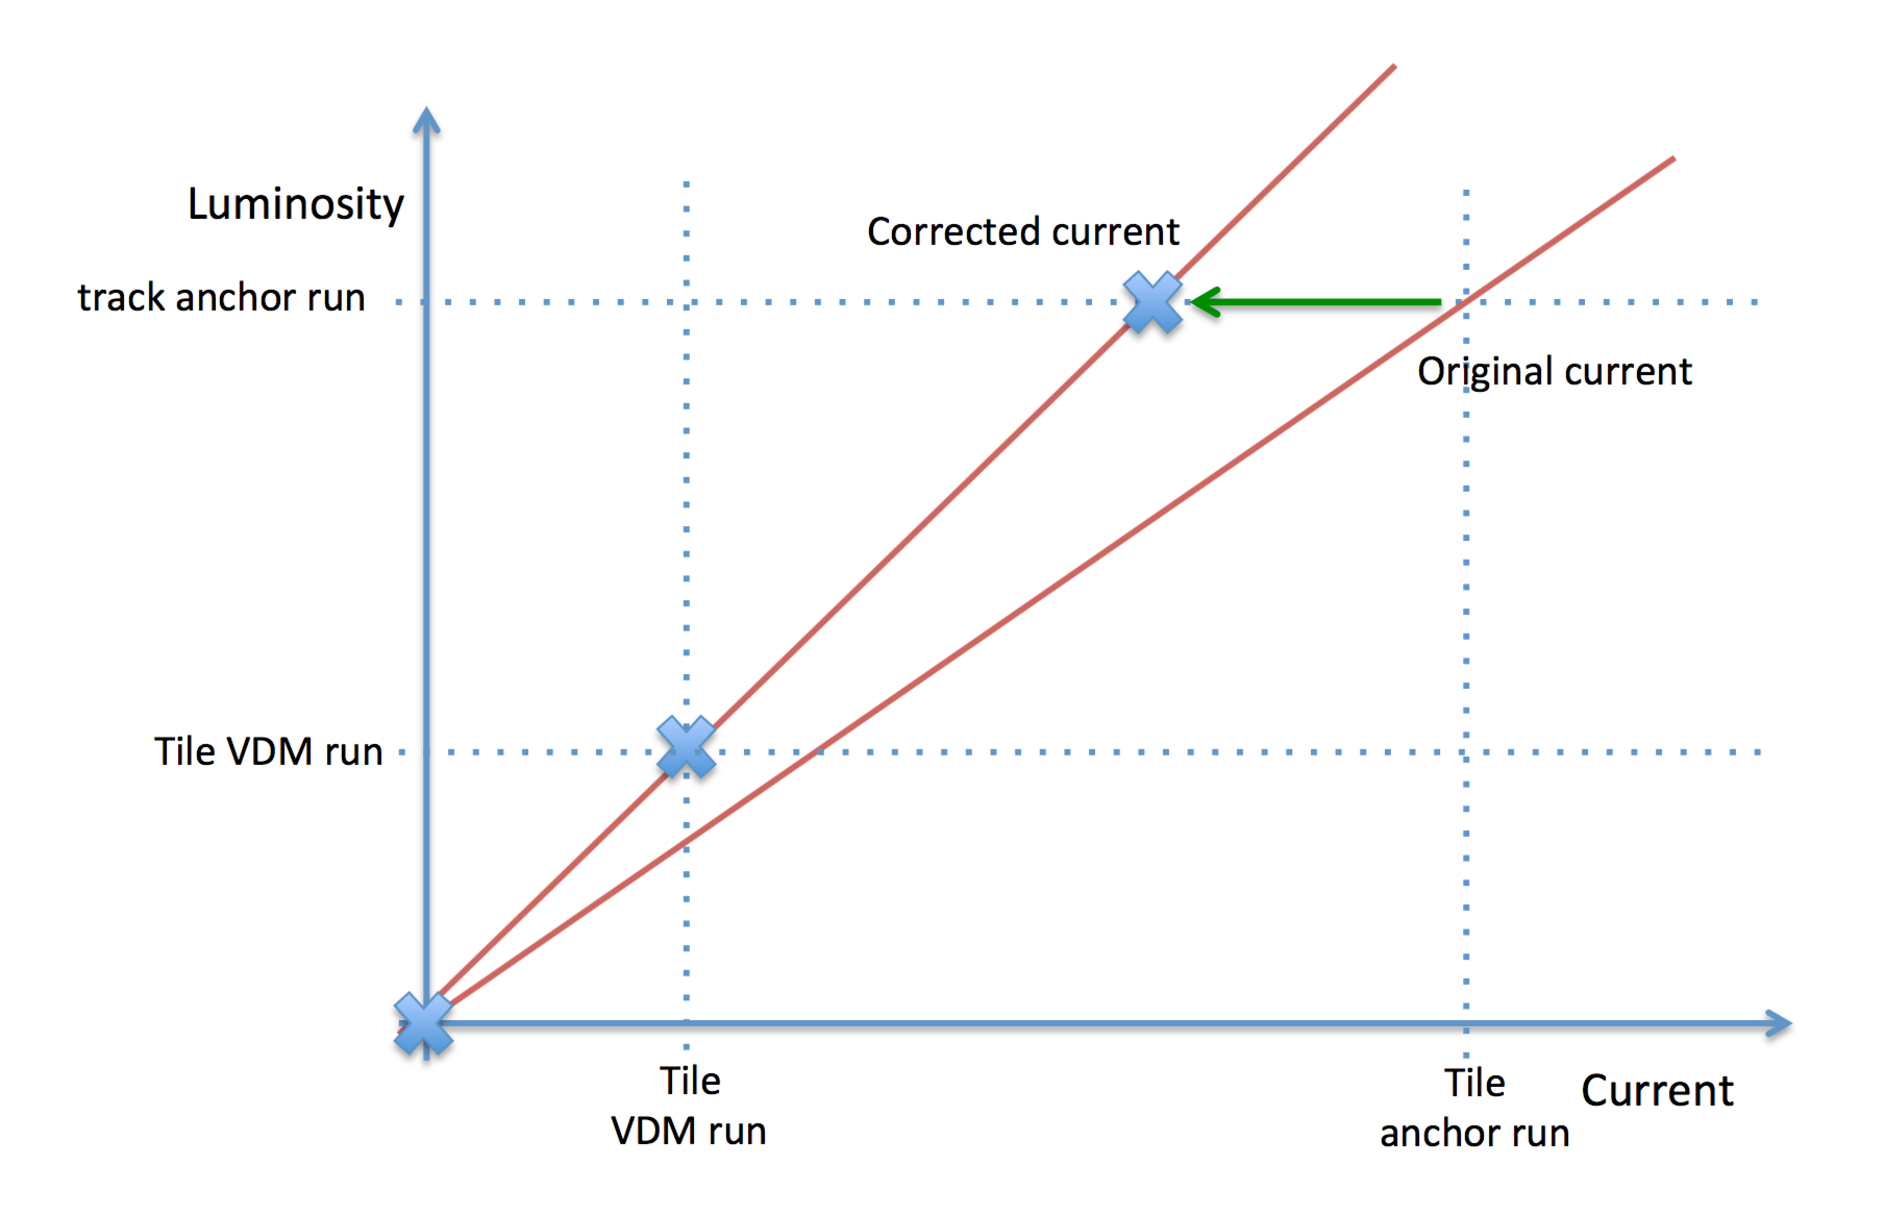
\includegraphics[width=0.65\textwidth]{figures/pmt_response/sketch.pdf}}
\caption{Schematic effect of the correction of the \gls{pmt} response on the \gls{tilecal} luminosity measurement.}
\label{fig:apppmt:sketch}
\end{figure}


\section{Conclusion}

The effect a non-linearity in the \gls{pmt} response with the increase in luminosity in the calibration transfer uncertainty from 
\gls{tilecal} has been studies. 
The calibration transfer uncertainty is one of the major sources of uncertainty in the \gls{atlas} luminosity 
measurement, and it has a relevant impact for analyses that rely on a precise luminosity measurement. 
A correction has been derived, that allowed to reduce the calibration transfer uncertainty by XX \%.
This correction has been applied to the computation of the luminosity uncertainty released in March 2018, 
leading to a total luminosity uncertainty of 2.4\% on the 2017 data-taking periods. 


